\subsection{Implementierung und Umsetzung}
\label{subsec:03implementierung}
Die Struktur des Algorithmus der Personenverfolgung mit ihren jeweiligen Modulen ist in Abbildung \ref{fig:personenverfolgung-struktur} dargestellt.
\begin{figure}[btp]
	\centering
	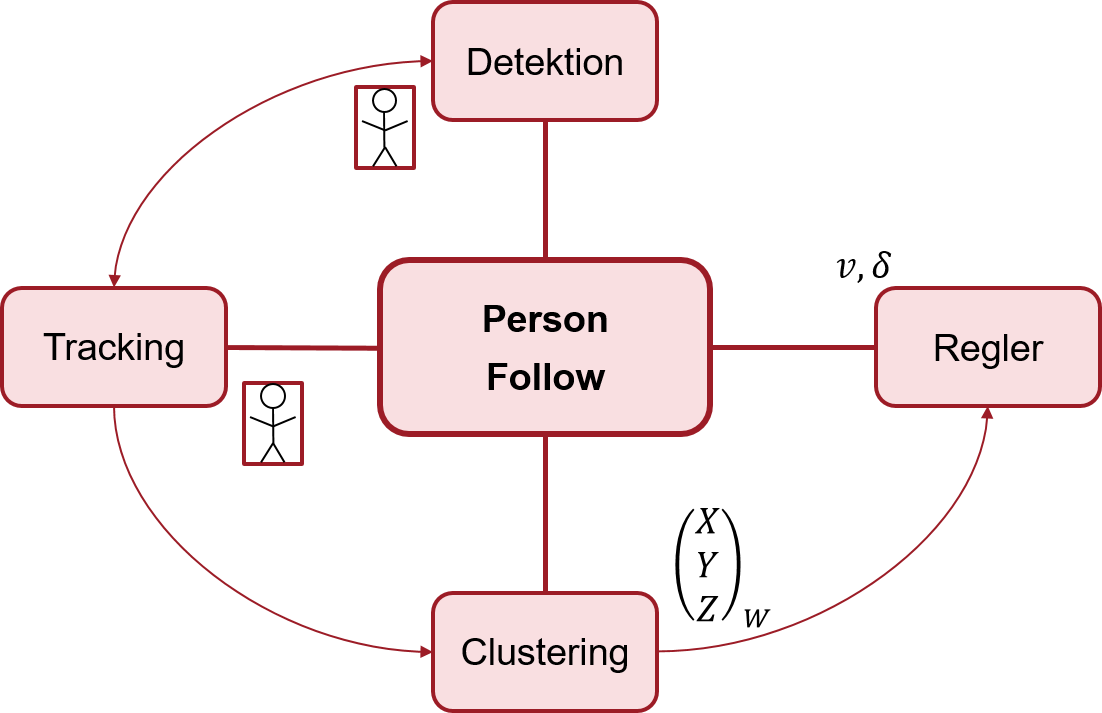
\includegraphics[width=.7\textwidth]{./pics/personenverfolgung_output.png}
	\caption{Struktur der Personenverfolgung mit jeweiligen Modulen.}
	\label{fig:personenverfolgung-struktur}
\end{figure}
Dabei ist anhand der Pfeilrichtungen gut zu erkennen, wie die einzelnen Module miteinander verkn�pft sind. Anfangs wird mittels der Detektion eine Person im Farbbild detektiert und als Zielperson f�r die Anfahrt festgelegt. Letzteres wird durch die Erstellung einer Bounding Box um die Person erreicht. Da diese Detektion ziemlich rechenaufw�ndig ist, w�rde die Bildrate der Kamera bei stetiger Detektion stark abfallen. Daher ist die Kombination mit einem Tracker notwendig. Dieser wird aktiviert, sobald eine Personendetektion erfolgt und bekommt die entsprechende Bounding Box �bergeben. Da Trackeralgorithmen grunds�tzlich mit einem gewissen Drift der Position der Person bzw. des Objektes einhergehen ist eine Umschaltung zur Detektion nach einer gewissen Zeit sinnvoll, um die Korrektheit der Bounding Box wiederherzustellen. Somit findet ein stetiger Wechsel beider Module statt. Im Modul Clustering erfolgt die Berechnung der Personenkoordinaten. Dazu geschieht eine Projektion der Bounding Box vom Farbbild in das Tiefenbild. Innerhalb der projizierten Bounding Box wird die Person von der Umgebung extrahiert und ihre Tiefe bestimmt. Mithilfe dieser und der Projektionsmatrix erfolgt die Berechnung der Koordinaten der Person. Diese bekommt der Regler �bergeben, welcher daraus das finale Ziel berechnet und einen entsprechenden Lenkwinkel $\theta$ und eine entsprechende Geschwindigkeit $v$ vorgibt.